%\documentclass[1p]{elsarticle}

\documentclass[10pt,twoside]{article}
\usepackage{amsfonts}
\usepackage{amsmath}
\usepackage{amssymb}
\usepackage[spanish]{babel}
\selectlanguage{spanish}
\usepackage[utf8]{inputenc}
\usepackage{graphicx}
\usepackage{latexsym}
\usepackage{booktabs}
\usepackage[pdftex=true,colorlinks=true,plainpages=false]{hyperref}
\usepackage[top=2.25cm,bottom=2cm,left=2cm,right=2cm,footskip=1cm,headheight=1cm,headsep=0.75cm,textwidth=1cm]{geometry}
\usepackage{fancyhdr}
\usepackage{setspace}
\usepackage{titlesec}
\usepackage{listings}
\usepackage{colortbl}
\usepackage{float}
%\floatstyle{boxed} 
\restylefloat{figure}
\usepackage[section]{placeins}
\usepackage{titlesec}
\titlelabel{\thetitle.\quad}

%\usepackage[affil-it]{authblk}
%\usepackage{color}
\usepackage{array}
\usepackage{colortbl}

\DeclareMathOperator*{\minimize}{\bf min}
\DeclareMathOperator*{\maximize}{\bf max}
\DeclareMathOperator*{\st}{\bf s.t.}
\DeclareMathOperator*{\argmax}{argmax}
\DeclareMathOperator*{\argmin}{argmin}
\DeclareMathOperator*{\diam}{diam}
\DeclareMathOperator*{\diag}{diag}

\newcommand{\balpha}{\bm{\alpha}}
\newcommand{\bbR}{\mathbb{R}}
\newcommand{\uno}{\mathbf{1}}
\newcommand{\by}{\mathbf{y}}
\newcommand{\bx}{\mathbf{x}}
\newcommand{\bxi}{\mathbf{x}_i}
\newcommand{\bz}{\mathbf{z}}
\newcommand{\bzi}{\mathbf{z}_i}
\newcommand{\bzj}{\mathbf{z}_j}
\newcommand{\bd}{\mathbf{d}}
\newcommand{\be}{\mathbf{e}}
\newcommand{\bu}{\mathbf{u}}
\newcommand{\bv}{\mathbf{v}}
\newcommand{\bone}{\mathbf{1}}
\newcommand{\bc}{\mathbf{c}}
\newcommand{\bp}{\mathbf{p}}
\newcommand{\bK}{\bm{K}}
\newcommand{\bY}{\bm{Y}}
\newcommand{\bI}{\bm{I}}
\newcommand{\cI}{\mathcal{I}}
\newcommand{\cB}{\mathcal{B}}
\newcommand{\cX}{\ensuremath{\mathcal{X}}}
\newcommand{\cY}{\ensuremath{\mathcal{Y}}}
\newcommand{\cZ}{\ensuremath{\mathcal{Z}}}
\newcommand{\cS}{\ensuremath{\mathcal{S}}}
\newcommand{\cO}{\ensuremath{\mathcal{O}}}
\newcommand{\cC}{\ensuremath{\mathcal{C}}}
\newcommand{\bZ}{\bm{Z}}

\newcommand{\ch}{ch}
\newcommand{\tset}{\ensuremath{\{(\bx_i,y_i): i \in \mathcal{I}\}}}
\newcommand{\indexset}{\ensuremath{\mathcal{I} = \{1,2,\ldots,m\}}}
\newcommand{\sgn}{\ensuremath{\mbox{sgn}}}

\newtheorem{proposition}{Proposition}
\newtheorem{theorem}{Theorem}
\newtheorem{lemma}{Lemma}
\newtheorem{corollary}{Corollary}

\newtheorem{definition}{Definition}
\newtheorem{remark}{Remark}
\newtheorem{assumption}{Assumption}
\newcommand{\HRule}{\rule{\linewidth}{0.25mm}}


\begin{document}
\begin{center}
~\\[-1.5cm]

\textsc{ \scalebox{1} Universidad Técnica Federico Santa María}\\[0.1cm]
\textsc{ \scalebox{1} Análisis Numérico - Departamento de Matemáticas}\\[0.1cm]
\textsc{1er Semestre 2018\\}

\HRule \\[0.1cm]
{\Large\textsc{ Tarea Laboratorio $N^{\circ} 1$ - Sistemas Lineales\\}}
\HRule \\[0.1cm]
\vspace{3mm}

\vspace{0.1mm}
Profesor: Gredy Jhovanny Salmerón Casco\\
\vspace{0.1mm}

\vspace{0.1mm}
Ayudante Laboratorio: Leonardo Aguero\\
\vspace{3mm}

\textbf{FECHA DE ENTREGA: Miércoles 16 de Mayo de 2018\\} 

\end{center}
\begin{flushleft}

\vspace{3mm}
\textbf{Nombre: Pablo Issai Calcumil Alarcón\\}
\vspace{3mm}

\textbf{Rol: 201673563 - 1\\}
\vspace{3mm}

\textbf{Paralelo Cátedra: 201\\}
\vspace{3mm}
\end{flushleft}

\section{Problema 1}

\begin{flushleft}
Primero que nada, se propone el sistema de ecuaciones, quedando de la siguiente manera:

\begin{center}
$34i_a - 30i_b = 6$

$30i_a - 66i_b + 20i_c = 0$

$ 20i_b - 25i_c = 40$

\end{center}

De forma matricial tenermos que:
\begin{center}

$
\begin{pmatrix}
  34  & -30 &  0  \\
   30  & -66 &  20  \\
   0 &  20 &  -25 
 \end{pmatrix}
 \begin{pmatrix}
  i_a \\
   i_b \\
   i_c
  \end{pmatrix}
   = \begin{pmatrix}
  6 \\
   0 \\
   40  
  \end{pmatrix}
$
\end{center}

1) Para resolver este sistema de ecuaciones, se utilizará el método LU, el cual forma 2 sistemas de ecuaciones que son
$Ly = b $ y $Ux = y$
, donde L es una matriz triangular inferior y U triangular superior.

\begin{center}
Primero se resuelve ek sistema $Ly = b$:
\vspace{1.5mm}

$
\begin{pmatrix}
  1  & 0 &  0  \\
   0.88235  & 1 &  0  \\
   0 &  -0.50595 &  1 
 \end{pmatrix}
 \begin{pmatrix}
  y_a \\
   y_b \\
   y_c
  \end{pmatrix}
   = \begin{pmatrix}
  6 \\
   0 \\
   40
  \end{pmatrix}
$

\vspace{3mm}
Ahora se resuelve el sistema $Ux = y$ :
\vspace{1.5mm}

$
\begin{pmatrix}
  34  & -30 &  0  \\
   0  & -39.52941 &  20  \\
   0 &  0 &  -14.88095
 \end{pmatrix}
 \begin{pmatrix}
  i_a \\
   i_b \\
   i_c
  \end{pmatrix}
   = \begin{pmatrix}
   6 \\
   -5.2941 \\
   37.3214  
  \end{pmatrix}
$
\end{center}

2) Los resultados del sistema son:
\begin{center}
$
\begin{pmatrix}
  i_a \\
   i_b \\
   i_c
  \end{pmatrix}
   = \begin{pmatrix}
  -0.825 \\
   -1.135 \\
   -2.508   
  \end{pmatrix}
$

Con estos valores es fácil notar que el sistema de giro de la corriente en las mallas no fue el correcto, por ende, los verdaderos valores de estos son: $i_a = 0.825, \hspace{2mm} i_b = 1.135 \hspace{2mm} y\hspace{2mm} i_c = 2.508$.
\end{center}

3) Para calcular la Potencia Disipada utilizamos $P = R \cdot i^2$, los valores se representan en la siguiente tabla::

\begin{center}
\begin{tabular}{l|lllllllll}
 & $R_{11}$& $R_{12}$& $R_{13}$& $R_{21}$& $R_{22}$& $R_{23}$& $R_{31}$& $R_{32}$& $R_{33}$ \\\hline
 Potencia &  23.1413 & 20.4188 & 0 & 38.6468 & 85.0229 & 25.7645 & 0 & 125.8013 & 157.2516  
\end{tabular}

\end{center}


\end{flushleft}


\clearpage
\section{Problema 2 Matemáticas}
\centering

\begin{flushleft}
1) Antes de presentar el sistema de ecuaciones, se cambiarán los nombres a las variables para simplificar trabajo:
\begin{center}
$T_{1,1} = A; \hspace{2mm} T_{1,2} = B; \hspace{2mm} T_{1,3} = C;\hspace{2mm}T_{2,1} = D;\hspace{2mm}T_{2,2} = E;\hspace{2mm}T_{2,3} = F;\hspace{2mm}T_{3,1} = G;\hspace{2mm}T_{3,2} = H;\hspace{2mm}T_{3,3} = I.$
\end{center}
Ahora con estos cambios se presenta el sistema de ecuaciones, formados por la ecuación de cada nodo, desde el (1,1) al (3,3):

\begin{center}
$-4A + B + D = -75$

$A - 4B + C + E = -75$

$B - 4C + F = -175$

$A - 4D + E + G = 0$

$B + D - 4E + F + H = 0$

$C + E - 4F + I = -100$

$D - 4G + H = -50$

$E + G - 4H + I = -50$

$F + H - 4I = -150$

\end{center}

2) Escribiendo de forma matricial estas ecuaciones, se tiene:

\end{flushleft}

$ 
 \begin{pmatrix}
  -4  & 1 &  0 &  1 &  0 &  0 &  0 &  0 &  0  \\
   1  & -4 &  1 &  0 &  1 &  0 &  0 &  0 &  0  \\
   0 &  1 &  -4 &  0 &  0 &  1 &  0 &  0 &  0  \\
   1  & 0 &  0 &  -4 &  1 &  0 &  1 &  0 &  0  \\
   0  & 1 &  0 &  1 &  -4 &  1 &  0 &  1 &  0  \\
   0 &  0 &  1 &  0 &  1 &  -4 &  0 &  0 &  1  \\
   0  & 0 &  0 &  1 &  0 &  0  & -4 &  1 &  0  \\ 
   0 &  0  & 0 &  0 &  1 &  0 &  1 &  -4 &  1  \\
   0 &  0  & 0 &  0 &  0 &  1 &  0 &  1 &  -4  
 \end{pmatrix}
 \begin{pmatrix}
  A \\
   B \\
   C \\
   D \\
   E \\
   F \\
   G \\
   H \\
   I  
  \end{pmatrix}
   = \begin{pmatrix}
  -75 \\
   -75 \\
   -175 \\
   0 \\
   0 \\
   -100 \\
   -50 \\
   -50 \\
   -150 
  \end{pmatrix}
 $
 
\vspace{2.5mm}

Se resuelve por el método LU, ya que al estar pivoteada, esta es muy fácil de realiza. Se podría por Cholesky si se multiplicara tanto A, como b por -1. Jacobi y Gauss-Seidel llegan a los mismos valores ya que su $\rho (T)<1$, es decir convergen, pero no se realizará así por no tener tolerancia. Los valores a los que se llega son:

\vspace{2.5mm}
$
\begin{pmatrix}
  A \\
   B \\
   C \\
   D \\
   E \\
   F \\
   G \\
   H \\
   I  
  \end{pmatrix}
   = \begin{pmatrix}
  42.857 \\
   63.170 \\
   78.571 \\
   33.259 \\
   56.250 \\
   76.116 \\
   33.929 \\
   52.455 \\
   69.643  
  \end{pmatrix}
 $

\begin{flushleft}
3) Este es el gráfico de la placa:
\begin{figure}[H]
  \caption{Gráfico Matriz.}
  \centering
    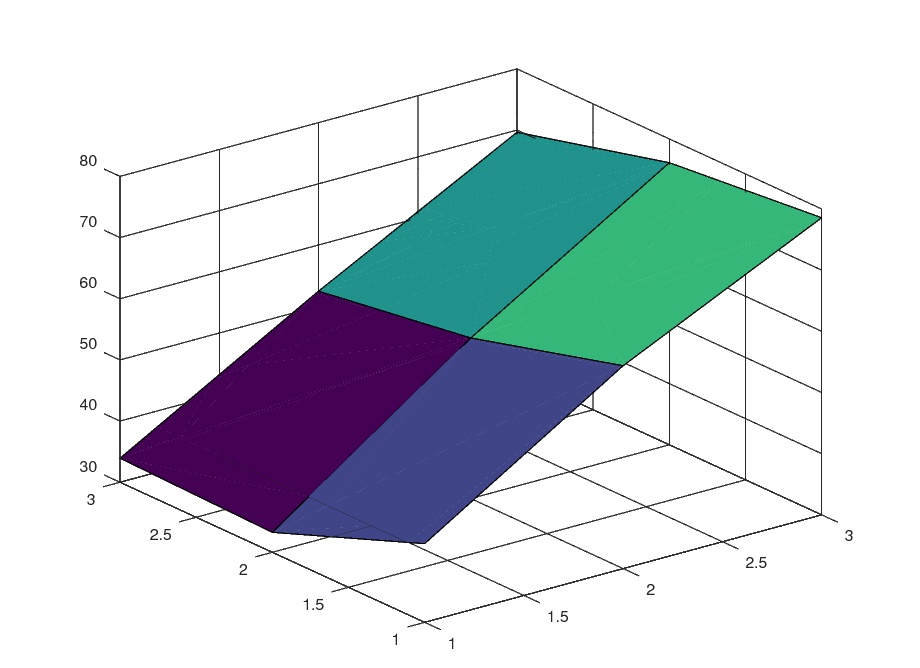
\includegraphics[width=0.9\textwidth]{Grafico}
\end{figure}
\end{flushleft}


\clearpage
\section{Problema 3}

\begin{flushleft}
\hspace{12mm}Se tiene el sistema
( $A x = b $ ).En donde el sistema lo constituye la matriz A, que esta formada por la función Trid(a, b, c, n) en donde a son los valores de la diagonal, b son los superiores y c los inferiores, y n la dimensión de la matriz cuadrada. Por otro lado, b esta formada por la función Pisano(n, d), que es dada por la función Fib(n) (secuencia de Fibonacci), donde con n se forma un vector columna de nx1 y d es el número con el cual se forma el modulo.\\
\end{flushleft}

Por términos de espacio, solo se pondrán en este informe la primera matriz y el primer vector, con su respectiva solución al sistema.


\begin{flushleft}
En el primer caso se utilizó: Trid(8, 4, 3, 10) y Pisano(10, 5). Formando lo siguiente:
\end{flushleft}

\vspace{5mm}
$
A = 
 \begin{pmatrix}
  8  & 4 &  0 &  0 &  0 &  0 &  0 &  0 &  0 &  0 \\
   3  & 8 &  4 &  0 &  0 &  0 &  0 &  0 &  0 &  0 \\
   0 &  3 &  8 &  4 &  0 &  0 &  0 &  0 &  0 &  0 \\
   0  & 0 &  3 &  8 &  4 &  0 &  0 &  0 &  0 &  0 \\
   0  & 0 &  0 &  3 &  8 &  4 &  0 &  0 &  0 &  0 \\
   0 &  0 &  0 &  0 &  3 &  8 &  4 &  0 &  0 &  0 \\
   0  & 0 &  0 &  0 &  0 &  3  & 8 &  4 &  0 &  0 \\ 
   0 &  0  & 0 &  0 &  0 &  0 &  3 &  8 &  4 &  0 \\
   0 &  0  & 0 &  0 &  0 &  0 &  0 &  3 &  8 &  4 \\
   0  & 0 &  0 &  0 &  0 &  0 &  0 &  0 &  3 &  8 
 \end{pmatrix}
  ; b = \begin{pmatrix}
  1 \\
   1 \\
   2 \\
   3 \\
   0 \\
   3 \\
   3 \\
   1 \\
   4 \\
   0 
  \end{pmatrix}
 $
 \vspace{5mm}
 
 Este sistema por medio del método LU da las siguiente soluciones: 
 
 \vspace{3mm}
 X = 
 $
 \begin{pmatrix}
 0.047114 \\
   0.155773 \\
  -0.096881 \\
   0.576932 \\
  -0.331203 \\
   0.229707 \\
   0.538988 \\
  -0.500257 \\
   0.846272 \\
  -0.317352
 \end{pmatrix}
$

 \vspace{5mm}
 
\begin{flushleft}
1) Se tiene que solo en el caso 2, la matriz es simétrica, es decir, al formar la matriz A = Trid(10, 3, 3, 100), por otro lado, se tiene que en el caso 1 y caso las matrices tienen valores propios positivos, pero como en el caso 1 no es simetrica, se puede decir que solo el caso 2 la matriz es definida positiva.
\end{flushleft}

Valores Propios (caso 1)=
 $
 \begin{pmatrix}
 1.3524 \\
    2.1716 \\
    3.4630 \\ 
    5.1219 \\
    7.0140 \\
   14.6476 \\
   13.8284 \\
    8.9860 \\
   12.5370 \\
   10.8781
 \end{pmatrix}
$

 \vspace{5mm}
 
\begin{flushleft}
2) Se sabe que el método de Cholesky, es: \[A = L L^{t}\] 
Esto lo realiza para matrices que son simétricas. Dicho esto, en los casos 1 y 3, (A = Trid(8, 4, 3, 10) y A = Trid(10, 5, 6, 100) respectivamente), el método de Cholesky no es efectivo, ya que cambia la matriz A y resuelve un sistema de ecuaciones distinto al que se requiere.

\vspace{5mm}

3) Se mostrarán solo los resultados del caso 1:
\end{flushleft}

Solución con Cholesky (caso 1) =  $
 \begin{pmatrix}
  0.098127 \\
   0.071662 \\
   0.044107 \\
   0.477385 \\
  -0.317133 \\
   0.368303 \\
   0.334991 \\
  -0.261613 \\
   0.695977 \\
  -0.260991 
 \end{pmatrix}
$

\begin{flushleft}
Se puede notar que está la diferencia con la solución dada en un principio, esto es por lo dicho anteriormente. El único caso en donde las soluciones son iguales es en el caso 2.

\vspace{5mm}

4) Solución presentada en el principio de la respuesta al problema 3. Si se puede utilizar en todos los casos, ya que tienen una muy buena estabilidad por estar pivoteada la matriz A en cada caso.
Acá se presenta los tiempos de ejecución (en segundos), de los métodos LU y Cholesky tanto para el caso 1, 2 y 3
\[t_{LU1} = 0.011510 \hspace{3mm}t_{Cho1} = 0.010742 \hspace{3mm}t_{LU2} = 0.71319\hspace{3mm}t_{Cho2} = 3.6419\hspace{3mm}t_{LU3} = 0.71232\hspace{3mm}t_{Cho3} = 3.8544\]

\vspace{5mm}

5)Las soluciones por los métodos de Jacobi y Gauss-Seidel son:

\end{flushleft}
Jacobi (caso1)
$
 \begin{pmatrix}
  0.047114 \\
   0.155773 \\
  -0.096881 \\
   0.576932 \\
  -0.331203 \\
   0.229708 \\
   0.538988 \\
  -0.500256 \\
   0.846272 \\
  -0.317352 
 \end{pmatrix}
$
\hspace{6mm} GS (caso 1)=
$
 \begin{pmatrix}
  0.047112 \\
   0.155775 \\
  -0.096883 \\
   0.576933 \\
  -0.331204 \\
   0.229708 \\
   0.538988 \\
  -0.500256 \\
   0.846272 \\
  -0.317352 
 \end{pmatrix}
$

\begin{flushleft}
Por otro lado, cabe decir que estos metodos no pueden ser utilizados para el caso 3, ya que como $\rho (T_J) > 1$ y $\rho (T_{GS}) > 1$ estas divergen, por otro lado, para los casos que convergen, sus tiempos en ejecución son:

\[t_{J1} = 0.019604 \hspace{3mm}t_{GS1} = 0.090034 \hspace{3mm}t_{J2} = 0.57345\hspace{3mm}t_{GS2} = 3.7573 \]
\end{flushleft}

\clearpage

\end{document}